	\documentclass{procDDs}

\usepackage[utf8]{inputenc}                                                 % load packages only if necessary
\usepackage[english, russian]{babel}
                                               

\title{Reconstruction of the Seabottom Reflection Coefficient}

\author{\textbf{Evgeny O. Kovalenko}, Igor V. Prokhorov, Andrey A. Sushchenko}% List of authors with the
{Institute for Applied Mathematics, FEB RAS, Vladivostok, Russia, \\ 
Far Eastern Federal University, Vladivostok, Russia}                 % same affiliation,
                                                  % lecturer given in bold
{kovalenko.eo@dvfu.ru, sushchenko.aa@dvfu.ru}                                   % e-mail of lecturer
%
%                                                 % it is important not to have
%                                                 % blank lines between the
%                                                 % \author and \coauthor
%

\begin {document}

\maketitle

\index{Kovalenko, E.O.}                              % write this for each author
\index{Prokhorov, I.V.}                              % to generate the index
\index{Sushchenko, A.A.}   
                          %
\def\k{\mathbf{k}}
\def\n{\mathbf{n}}
\def\x{\mathbf{x}}
\def\y{\mathbf{y}}
\def\r{\mathbf{r}}
\def\p{\mathbf{|}}
\def\z{\mathbf{z}}
\def\V{\mathbf{V}}
\def\Vt{\mathbf{V}t}
\def\exp{\text{exp}}

\begin{abstract}
   The kinetic model, describing sound propagation in the ocean with diffuse reflection by Lambert's cosine law on the bottom surface, is considered. Based on it the inverse problem of bottom scattering reconstruction is formulated. Обратная задача сведена к нахождению решения интегрального уравнения первого рода.
   Предложен итерационный алгоритм для нахождения решения обратной задачи и проведены численные эксперименты по восстановлению коэффициента донного рассеяния при различной ширине диаграммы направленности. 
\end{abstract}

\section{Introduction}

\begin{figure}[h!]\center
	
	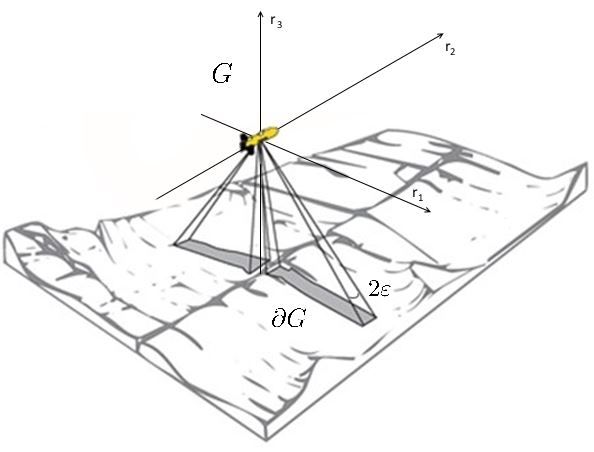
\includegraphics[width=1\linewidth]{img/gbo.jpg}
	\caption{АНПА с ГБО на борту}
	\label{ris:dno}
\end{figure}

Since the beginning of the 20th century, research on the mapping of the seabed is relevant. All methods base on sending and receiving signal. The basis of the developed methods for identification of the scattering coefficient of the seabottom is principle of radiation and detection of signal. 
В настоящее время особенно актуальна задача зондирования морского дна на основе данных, полученных  гидролокатором бокового обзора. В работах []  построены кинетические модели для процесса ГБО-зондирования морского в приближении однократного рассеяния и узкой диаграммы направленности.   Проведен  анализ влияния объемного рассеяния и ширины диаграммы направленности приемной антенны на качество восстановления гидролокационного изображения.   

Увеличение ширины диаграммы направленности и длительности импульса источника приводит к размытию гидролокационных изображению морского дна, полученных непосредственно с гидролокатора бокового обзора.
Проблема фокусировки размытых ГБО-изображений сведена к решению интегрального уравнения первого рода.
Для решения интегрального уравнения предложен итерационный метод Зейделя. Проведены численные эксперименты при различной ширине диаграммы направленности приемной антены ГБО.




\section{Formulation of the problem}
Propagation of acoustic waves on the tens order kHz frequencies in the fluctuating ocean is described by radiation
transfer equation\cite{p11},\cite{p12}:

A long formula:
\begin{multline}
	\label{model}
	\frac{1}{c} \frac{\partial I}{\partial t} + \k \cdot \nabla I(\r,\k,t) + 
	\mu I(\r,\k,t) = \\ J(\r,\k,t),
\end{multline}

here $\r \in \mathbb{R}^3, t \in [0, T]$ and wave vector $\k$ belongs to the unit sphere $\Omega := \{\k \in \mathbb{R}^3: |\k| = 1\}$. The function $I(\r,\k, t)$ denotes the wave energy of flux density at time $t$  at the point $\r$ which propagates in the direction $\k$  with velocity $c$. $\mu$ and $\sigma$ denote the attenuation and the scattering coefficients, respectively, and the function $J$ describes the sources of
wave field.

Sonar signal is propagated in the medium $G:=\{\r \in \mathbb{R}^3:r_3 > -l\}$, which is top half-space bounded by the surface $\partial G = \gamma := \{\y \in \mathbb{R}^3: y_3 = -l \}$, interpreted as the bottom of the ocean. и пусть $\textbf{n}(\y)$ --- внешняя нормаль к  границе области $G$. 



Further, authors consider the case of an isotropic pointwise source which moves with constant velocity $V$ along $r_2$ axis and emits a pulse parcels in times $t_i$, $\overline{1,m}$ with intensity $J_i$, respectively: 
\begin{equation}
	\label{source}
	J(\r,\k, t) = \delta(\r - \V t)\sum\limits_{i=0}^{m} J_i \frac{ \chi_{[-\frac{\Delta}{2};\frac{\Delta}{2}]}(t-t_i)}{\Delta}.
\end{equation}
Here, $\delta$ denotes Dirac delta function, $\chi_{[a,b]}$ is characteristic function of interval $[a,b]$.

Assume, sources in medium are missing before initial time
\begin{equation}
	\label{init_cond}
	I\rvert_{t=0}=0.
\end{equation}

Let, $\Omega^\pm := \{\k \in \Omega: \pm k_3 < 0\}$ then the reflective properties of $\partial G$  are determined by diffuse reflection by the Lambert’s cosine law:
\begin{equation}
	\label{boundary_condition}
	I(\y,\k) = \frac{\sigma_d}{\pi} \int\limits_{\Omega ^+}|\n(\y)\cdot \k'| I(\y,\k') d\k' ,
\end{equation}
where  $\y \in \partial G, \k \in \Omega^-$.


Let, $\Gamma := \{ (\Vt, \k, t): \k \in \Omega, t \in (0,T) \}$  then measuring of the receiving signal on $\Gamma$ is a sum of the signal, caused by the reflection from the bottom surface, and a signal scattered by the inhomogeneities of the medium $G$:
\begin{multline}
	\label{sum_sig}
	I^\pm(t) = \int_{\Omega} S^\pm(\k) I|_{\Gamma}(\Vt, \k, t)d\k.
\end{multline}
Here, $S^+(\k)$ and $S^-(\k)$ denote the directivity pattern of the receiving antenna on the starboard and portside, respectively. Further, authors consider the case of a narrow directivity pattern of the receiving antenna, focused on orthogonal plane to vehicle path:
\begin{equation}
\label{diagram}
S^\pm(\k) = \chi_{[0,\mp1]}(k_1)  \exp(-k_2^2/\varepsilon^2),
\end{equation}
where, $\varepsilon $ - angle of the width of directivity pattern.

\section{Determination of the bottom scattering coefficient}

Authors consider the case when the receiving antenna detects signals from one sensing interval only. 
The authors present a solution (\ref{model}) - (\ref{sum_sig}) as:
\begin{multline}
	I^\pm(t) = \frac{1}{\pi}\int\limits_{-1}^{1}\sigma_d(y_1,y_2) S^{\pm}(\k) \times \\ \times
	\frac{ cl^2J_i \exp(-\mu c(t-t_i))dk_2}{|\Vt_i-\y|^2|\y-\Vt|y_1(t-t_i)|k_2 \V-c|},
\end{multline}
here, $|\Vt - \y| = |\dfrac{c(t-t_i)}{2}(1+\dfrac{V^2}{c^2})|$, $|\x-\y| = |\dfrac{c(t-t_i)}{2}(1-\dfrac{V^2}{c^2})|$, $y_1 = \sqrt{|\Vt-\y|^2 - l^2}.$

\section{The Inverse Problem}
The inverse problem is determining the function $\sigma_d$ from equation (\ref{form})
\subsection{Narrow DP Approximation}
 For solving it author assume a narrow directivity pattern approximation:
\begin{equation}
S^{\pm}(\k) = \chi_{0,\mp1}(k_1)\delta(k_2)
\end{equation}
Thus, the solution of (7) is
\begin{equation}
	\label{sigma_form}
	\sigma_d \left( y_1, y_2 \right) = \frac{2\pi}{J_icl^2} l_i^4 y_1 \exp(2\mu l_i)I^\pm(t).
\end{equation}
Here, a slant range $l_i=c(t-t_i)/2$, and $y_1=\sqrt{l_i^2-l^2}, y_2=Vt_i$.

\subsection{Discrete Method}
С математической точки зрения уравнение (\ref{form}) относится к интегральному уравнению I рода относительно функции $\sigma_d$. Для его решения введём метод дискретизации. Тоесть определим области, в которых $\sigma_d$  константа. Так как $\sigma_d$ задана на множестве $\Gamma$, введём разбиение по осям $y_1, y_2$:
\begin{align}
	\{ \big( y_1^p, y_2^q \big) \in\gamma: y_1^p = ph, y_2^q = qh \}, \notag \\ 
	p \in \overline{1, H}, q \in \overline{1, M}, 
\end{align}
где $h$ - шаг сетки. Таким образом, в области, ограниченной точками $\big(y_1^p, y_2^q\big)$, $\big(y_1^{p+1}, y_2^q\big)$, $\big(y_1^p, y_2^{q+1}\big)$, $\big(y_1^{p+1}, y_2^{q+1}\big)$ $\sigma_d$ считается постоянной, и уравнение (\ref{form}) сводится к:
\begin{equation}
\label{invI}
	I(t_{ij}) = \sum \limits_{p=1}^{N} \sum \limits_{q=1}^{M} a_{ijpq}\sigma_d^{pq},
\end{equation}
where,
\begin{multline*}
t_{ij} = t_i+j\tau, \tau = \frac{\Delta_t}{M}, a_{ijpq} = \\ 
=  \int\limits_{-1}^{1}
\frac{cl^2J_i \exp(-\mu c(t-t_i))dk_2}{|\Vt_i-\y|^2|\y-\Vt|y_1(t-t_i)|k_2 \V-c|}, \\
\sigma_d^{pq} = \sigma_d(\textbf{y}^{pq}), \textbf{y}^{pq} = (y_1^p, y_2^q).
\end{multline*}
Уравнение (\ref{invI}) представляет собой $s$-диагональную СЛАУ. Параметр $s$ зависит от ширины диаграммы направленности приёмной и передающей антенн и длительности испускания сигнала. For solving SLE (\ref{invI}) authors use  Seidel's method.

\section{Numerical experiments}
В эксперименте рассматривались случаи фокусировки при разной ширине диаграммы направленности приемной антенны. В качестве нулевой итерации в методе Зейделя было взято решение, полученное по формуле (\ref{sigma_form}), изображенное на рисунках (\ref{ris:desc1} - \ref{ris:desc6}) над буквой а). В данном эксперименте рассмотрены случаи при диаграмме направленности равной 1, 2, 4, 8, 14, 40 градусов. Для оценки ЧЕГОТОТАМ было введено ЧТОТОТАМ(отклонение). 

Параметры, применяемые для построения изображения морского дна на основе реальных данных, получаемых с гидролокатора бокового обзора, представлены в таблице 1. Для решения задачи численного интегрирования применялся метод Монте-Карло. 
\begin{table}[!ht]
	\label{table:name}
	\center{\caption{Значения параметров для эксперимента }
	\begin{tabular}{|c|c|c|c|c|c|c|c|c|c|c|c|c|}
		\hline
			$\mu$,м$^{-1}$ & $\Delta t$,c & $c$,м/с & $J$ & $l$,м & $y_1$,м & $y_2$,м\\
			\hline
			0.018 & 0.4 & 1500 & 1 & 12 & [0,40] & [0, 40]\\ \hline
	\end{tabular}}	
\end{table}

Поверхность дна описывается функцией 
\begin{equation}
	\sigma_d=???
\end{equation}
 и изображена на рисунке \ref{ris:dno}.

\begin{figure}[h!]\center
	
		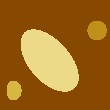
\includegraphics[width=0.3\linewidth]{img/dno.jpg}
	\caption{Точное решение}
	\label{ris:dno}
\end{figure}

\begin{figure}[h!]\center%---------------ONE DEGREE---------------
	\begin{tabular}{cccc}
		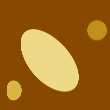
\includegraphics[width=0.2\linewidth]{img/5/1.jpg}&
		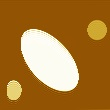
\includegraphics[width=0.2\linewidth]{img/5/3.jpg}&
		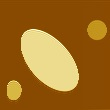
\includegraphics[width=0.2\linewidth]{img/5/4.jpg}&
		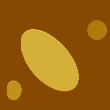
\includegraphics[width=0.2\linewidth]{img/5/6.jpg}\\
		a & b & c & d \\
		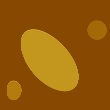
\includegraphics[width=0.2\linewidth]{img/5/7.jpg}&
		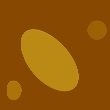
\includegraphics[width=0.2\linewidth]{img/5/8.jpg}&
		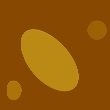
\includegraphics[width=0.2\linewidth]{img/5/8.jpg}&
		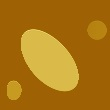
\includegraphics[width=0.2\linewidth]{img/5/9.jpg}\\
		\\
		e & f & g & h		
	\end{tabular}
	\caption{$1^\circ$}
	\label{ris:desc1}
\end{figure}
\begin{table}[h!]
	\label{table:desc1}
	\center{\caption{Нормы для $1^\circ \times$}
		\begin{tabular}{|c|c|c||c|c|c|}
			\hline
			& $||\Delta\sigma||_2$ & $||\Delta\sigma||_\infty$ &
			& $||\Delta\sigma||_2$ & $||\Delta\sigma||_\infty$ \\ \hline
			a & 0.0426 & 0.0749 & e &  0.0426 & 0.0749\\ \hline
			b & 0.0426 & 0.0749 & f &  0.0426 & 0.0749\\ \hline
			c & 0.0426 & 0.0749 & g &  0.0426 & 0.0749\\ \hline
			d & 0.0426 & 0.0749 & h &  0.0426 & 0.0749\\ \hline
	\end{tabular}}	
\end{table}
\begin{figure}[h!]\center%---------------TWO DEGREE---------------
	\begin{tabular}{cccc}
		
\includegraphics[width=0.2\linewidth]{img/6/1.jpg}&
		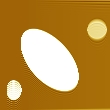
\includegraphics[width=0.2\linewidth]{img/6/3.jpg}&
		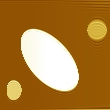
\includegraphics[width=0.2\linewidth]{img/6/4.jpg}&
		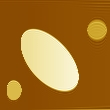
\includegraphics[width=0.2\linewidth]{img/6/5.jpg}\\
		a & b & c & d \\
		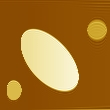
\includegraphics[width=0.2\linewidth]{img/6/5.jpg}&
		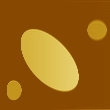
\includegraphics[width=0.2\linewidth]{img/6/6.jpg}&
		
\includegraphics[width=0.2\linewidth]{img/6/9.jpg}&
		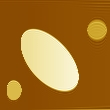
\includegraphics[width=0.2\linewidth]{img/6/5.jpg}\\
		e & f & g & h \\
	\end{tabular}
	\caption{$2^\circ$}
	\label{ris:desc2}
\end{figure}
\begin{table}[h!]
	\label{table:desc2}
	\center{\caption{Нормы для $2^\circ \times$}
		\begin{tabular}{|c|c|c||c|c|c|}
			\hline
			& $||\Delta\sigma||_2$ & $||\Delta\sigma||_\infty$ &
			& $||\Delta\sigma||_2$ & $||\Delta\sigma||_\infty$ \\ \hline
			a & 0.0426 & 0.0749 & e &  0.0426 & 0.0749\\ \hline
			b & 0.0426 & 0.0749 & f &  0.0426 & 0.0749\\ \hline
			c & 0.0426 & 0.0749 & g &  0.0426 & 0.0749\\ \hline
			d & 0.0426 & 0.0749 & h &  0.0426 & 0.0749\\ \hline
			
	\end{tabular}}	
\end{table}
\begin{figure}[h!]\center%---------------FOUR DEGREE---------------
	\begin{tabular}{cccc}
		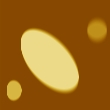
\includegraphics[width=0.2\linewidth]{img/7/1.jpg}&
		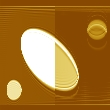
\includegraphics[width=0.2\linewidth]{img/7/3.jpg}&
		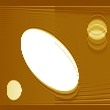
\includegraphics[width=0.2\linewidth]{img/7/4.jpg}&
		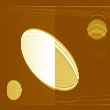
\includegraphics[width=0.2\linewidth]{img/7/5.jpg}\\
		a & b & c & d\\
		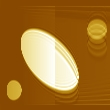
\includegraphics[width=0.2\linewidth]{img/7/6.jpg}&
		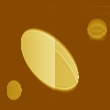
\includegraphics[width=0.2\linewidth]{img/7/7.jpg}&
		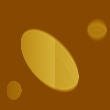
\includegraphics[width=0.2\linewidth]{img/7/8.jpg}&
		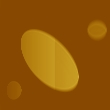
\includegraphics[width=0.2\linewidth]{img/7/9.jpg}\\
		e & f & g & h
	\end{tabular}
	\caption{$4^\circ$}
	\label{ris:desc3}
\end{figure}
\begin{table}[h!]
	\label{table:desc3}
	\center{\caption{Нормы для $4^\circ$}
		\begin{tabular}{|c|c|c||c|c|c|}
			\hline
			& $||\Delta\sigma||_2$ & $||\Delta\sigma||_\infty$ &
			& $||\Delta\sigma||_2$ & $||\Delta\sigma||_\infty$ \\ \hline
			a & 0.3333 & 0.1035 & e &  0.1653 & 0.0198\\ \hline
			b & 0.236 & 0.0627 & f &  0.1636 & 0.0266\\ \hline
			c & 0.2 & 0.0247 & g &  0.1819 & 0.0406\\ \hline
			d & 0.1634 & 0.0234 & h &  0.1983 & 0.0526\\ \hline
			
	\end{tabular}}	
\end{table}
\begin{figure}[h!]\center%---------------EIGHT DEGREE---------------
	\begin{tabular}{cccc}
		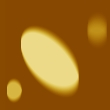
\includegraphics[width=0.2\linewidth]{img/9/1.jpg}&
		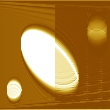
\includegraphics[width=0.2\linewidth]{img/9/3.jpg}&
		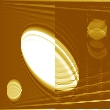
\includegraphics[width=0.2\linewidth]{img/9/4.jpg}&
		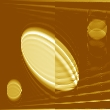
\includegraphics[width=0.2\linewidth]{img/9/5.jpg}\\
		a & b & c & d\\
		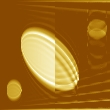
\includegraphics[width=0.2\linewidth]{img/9/6.jpg}&
		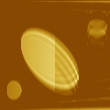
\includegraphics[width=0.2\linewidth]{img/9/7.jpg}&
		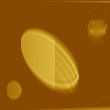
\includegraphics[width=0.2\linewidth]{img/9/8.jpg}&
		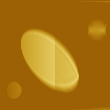
\includegraphics[width=0.2\linewidth]{img/9/9.jpg}\\
		e & f & g & h
	\end{tabular}
	\caption{$8^\circ$}
	\label{ris:desc4}
\end{figure}
\begin{table}[h!]
	\label{table:desc4}
	\center{\caption{Нормы для $8^\circ$}
		\begin{tabular}{|c|c|c||c|c|c|}
			\hline
			& $||\Delta\sigma||_2$ & $||\Delta\sigma||_\infty$ &
			& $||\Delta\sigma||_2$ & $||\Delta\sigma||_\infty$ \\ \hline
			a & 0.1959 & 0.0521 & e &  0.2 & 0.0299\\ \hline
			b & 0.2766 & 0.0424 & f &  0.1933 & 0.0324\\ \hline
			c & 0.2239 & 0.0319 & g &  0.1755 & 0.0399\\ \hline
			d & 0.1984 & 0.0291 & h &  0.1817 & 0.0477\\ \hline
			
	\end{tabular}}	
\end{table}
\begin{figure}[h!]\center%---------------FOURTEEN DEGREE---------------
	\begin{tabular}{cccc}
		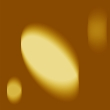
\includegraphics[width=0.2\linewidth]{img/13/1.jpg}&
		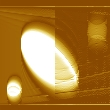
\includegraphics[width=0.2\linewidth]{img/13/3.jpg}&
		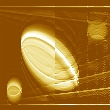
\includegraphics[width=0.2\linewidth]{img/13/4.jpg}&
		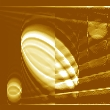
\includegraphics[width=0.2\linewidth]{img/13/5.jpg}\\
		a & b & c & d\\
		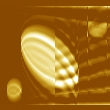
\includegraphics[width=0.2\linewidth]{img/13/6.jpg}&
		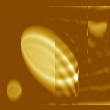
\includegraphics[width=0.2\linewidth]{img/13/7.jpg}&
		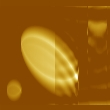
\includegraphics[width=0.2\linewidth]{img/13/8.jpg}&
		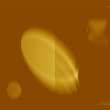
\includegraphics[width=0.2\linewidth]{img/13/9.jpg}\\
		e & f & g & h
	\end{tabular}
	\caption{$14^\circ$}
	\label{ris:desc5}
\end{figure}
\begin{table}[h!]
	\label{table:desc5}
	\center{\caption{Нормы для $14^\circ$}
		\begin{tabular}{|c|c|c||c|c|c|}
			\hline
			& $||\Delta\sigma||_2$ & $||\Delta\sigma||_\infty$ &
			& $||\Delta\sigma||_2$ & $||\Delta\sigma||_\infty$ \\ \hline
			a & 0.1926 & 0.0536 & e &  0.2225 & 0.0382\\ \hline
			b & 0.3106 & 0.0524 & f &  0.2 & 0.0355\\ \hline
			c & 0.3066 & 0.0428 & g &  0.2 & 0.0369\\ \hline
			d & 0.2505 & 0.0440 & h &  0.2 & 0.0423\\ \hline
			
	\end{tabular}}	
\end{table}
\begin{figure}[h!]\center%---------------FOUTY DEGREE---------------
	\begin{tabular}{cccc}
		
\includegraphics[width=0.2\linewidth]{img/17/1.jpg}&
		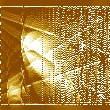
\includegraphics[width=0.2\linewidth]{img/17/3.jpg}&
		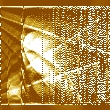
\includegraphics[width=0.2\linewidth]{img/17/4.jpg}&
		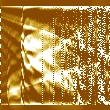
\includegraphics[width=0.2\linewidth]{img/17/5.jpg}\\
		a & b & c & d\\
		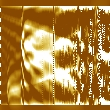
\includegraphics[width=0.2\linewidth]{img/17/6.jpg}&
		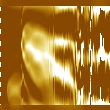
\includegraphics[width=0.2\linewidth]{img/17/7.jpg}&
		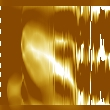
\includegraphics[width=0.2\linewidth]{img/17/8.jpg}&
		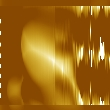
\includegraphics[width=0.2\linewidth]{img/17/9.jpg}\\
		e & f & g & h
	\end{tabular}
	\caption{$40^\circ$}
	\label{ris:desc6}
\end{figure}
\begin{table}[h!]
	\label{table:desc6}
	\center{\caption{Нормы для $40^\circ$}
		\begin{tabular}{|c|c|c||c|c|c|}
			\hline
			& $||\Delta\sigma||_2$ & $||\Delta\sigma||_\infty$ &
			& $||\Delta\sigma||_2$ & $||\Delta\sigma||_\infty$ \\ \hline
			a & 0.0886 & 0.4 & e &  0.1332 & 0.4\\ \hline
			b & 0.1438 & 0.4 & f &  0.1263 & 0.4\\ \hline
			c & 0.1444 & 0.4 & g &  0.1204 & 0.4\\ \hline
			d & 0.1384 & 0.4 & h &  0.1165 & 0.4\\ \hline
			
	\end{tabular}}	
\end{table}
 
\subsection{Subsection}

Body of subsection.

Numbered formula should be written as
\begin{equation}\label{key}                       % key is any name used
a+b=2.                                         % to refer to the formula
\end{equation}

The reference to such an equation should be as (\ref{key}).

A few formulae:
\begin{gather}                       % key is any name used
a+b=2,\label{key1}\\
c+d=3.\label{key2}
\end{gather}


Aligned formulae:
\begin{align}                       % key is any name used
A={}&\int_0^1f(x)\mathrm{d}x,\notag\\
&{}+a+b+c,\label{key3}\\
B={}&3.\label{key4}
\end{align}

A long formula:
\begin{multline}
D=a+b+c+e+\sum_{n=1}^\infty t_n\\
+f+\int_0^1g(x)\mathrm{d}x+q+h+y^2\\
-r-s-\sin(w).
\end{multline}
 
% See http://mirror.ctan.org/macros/latex/required/amslatex/math/amsldoc.pdf
% for more examples of AMS-LaTeX commands.
 
Citations are written as \cite{paper1}.           % paper1 is the name from
                                                  % \bibitem commands below



\section*{Acknowledgements}

Put acknowledgements in the last section, please do not use footnotes for that.

%  citations should be arranged by order of appearance

\begin {thebibliography}{9}

\bibitem{p1} Surname, I.\,I., Surname, I.\,I., 1998,
            Title of the reference,
            \emph{Journal}, Vol.\;{\bf 2}, pp.\;15--25.

\bibitem{p2} Surname, I.\,I., 2010, \textit{Title of Book}, Publisher, City.

\end{thebibliography}

\end {document}
